\chapter{Visualisation implementation}\label{C:sd}
This chapter discusses the implementation of the visulisation uisng the designs discussed previously. It details the tools used, the deliverables produced, and the problems encountered
%It details decisions made during the project such as choosing a viable framework, the choice of extending a previous system, platform choice, and designs of the actual system.   
\section{Tools and artifacts used}

\section{Technology choice}
Many technologies were looked into,experimented with, and the positives and negatives of each weighed up before a decision was made about which would be the choice for the visualisation. It came down to 3 potential technologies that would be suitable for the project, the next 3 subsections outline these in detail.

\subsubsection{D3 (Data Driven Documents)}
D3 is a JavaScript library that allows the displaying of data in dynamic graphics. Embedded
within an HTML web page, the JavaScript D3.js library uses pre-built JavaScript functions to
select elements, create Scalable Vector Graphic (SVG)[17] objects, style them, and add transitions,
dynamic effects and tooltips. Large datasets can be easily bound to SVG objects using
simple D3 functions to generate rich charts and diagrams. D3 was created because of the
need for a balance of expressiveness, efficiency, and accessibility that previous visualization
toolkits did not allow [4].

D3 allows the binding of input data to arbitrary input elements. This means that the exoplanet
dataset can easily be bound to SVG elements for creating visualizations. D3 adopts
the W3C Selectors API to identify document elements queried. This results in a rich but
concise selection method of elements in a visualisation.

D3 allows debugging thanks to Google chrome and other modern browsers development
tools. A downside to D3 is that it does not allow 3D diagrams, although it does allow
pseudo 3D by using the painter’s algorithm and 3D textures.

\subsubsection{Prefuse}
Prefuse is a set of software tools for creating rich interactive data visualizations [13]. The
Prefuse toolkit provides a visualization framework for Java. It supports a set of features
for visualizing and interacting with data. It provides optimized data structures for tables,
graphs, and trees. It can be used to build standalone applications, visual components embedded
in larger applications, and web applets. Prefuse to greatly simplifies the process
of representing and efficiently handling data, mapping data to visual representations (e.g.,
through spatial position, size, shape, color, etc), and interacting with the data.
To use Prefuse a basic familiarity with the Java is required, including setting up and building
Java projects. A knowledge of Swing or another similar user interface toolkit is also
useful for understanding some of the concepts behind Prefuse and for integrating Prefuse
visualizations into larger applications. Experience with database systems is also helpful. 
However the complexity of Prefuse means that the learning curve will be out of scope for
this project.

\subsubsection{Processing}
Processing is an open source programming language and development environment that was initially created to serve as a software
sketchbook and to teach the fundamentals of computer programming with a visual context.
Using processing would mean that the visualization could be built with Java while still using
a successful visualisation framework. The most complete existing visualization using
the same exoplanet dataset (Kepler Visualization Tool) is built using Processing.
Using this solution would involve learning the Processing language, however Processing
is a library built in Java so the syntax is the same. This means the learning curve should be shallow.
Using processing means that 3D elements could be included, this wouldnt be
possible with D3.

\subsubsection{Decision of technology}
The final decsion of techology was to use Processing, this is because it had many positive aspects that the others did not and minimal nigatives as the below table illistrates.
\clearpage
\begin{figure}[h!]
  \centering
      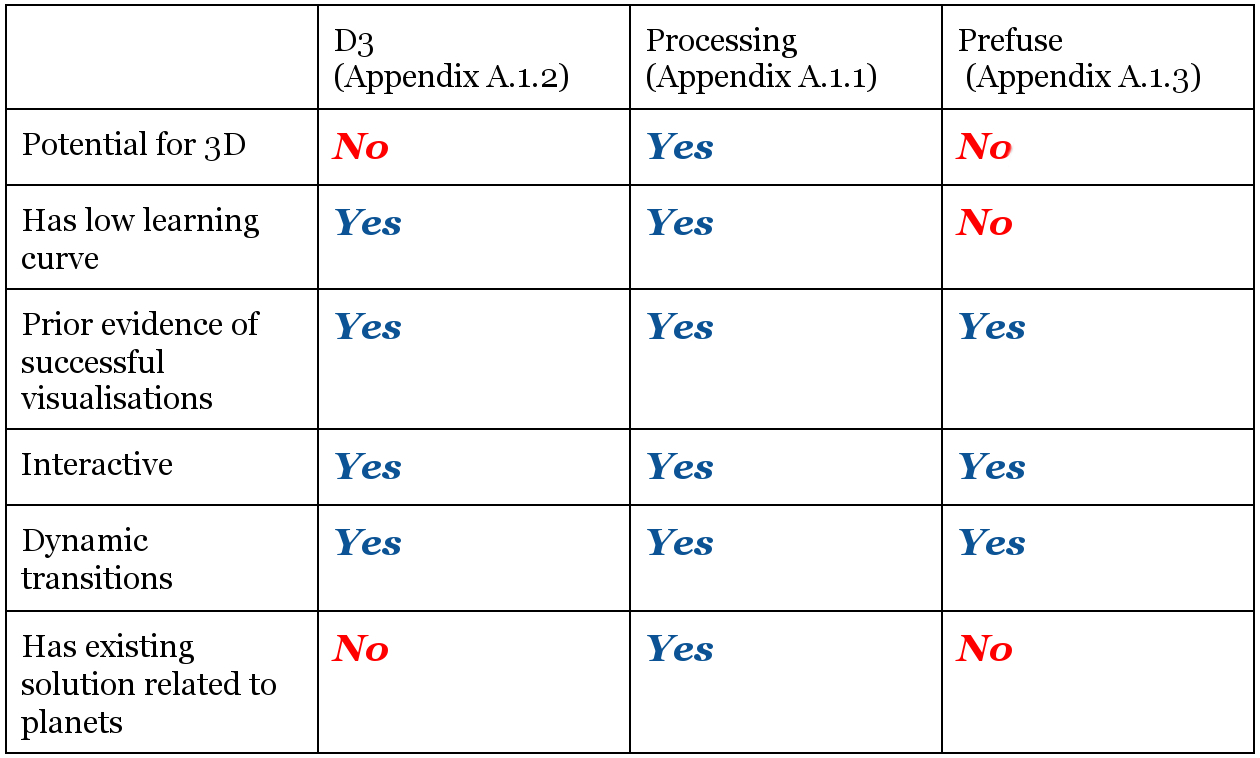
\includegraphics[width=0.8\textwidth]{images/table_technologies.jpg}
  \caption{Table of technology choices}
\end{figure}

As this project was created using Processing, it allowed me to extend the previous visualisation using the same data set, The Kepler Visualisation Tool \cite{kepler_github, kepler_article}. As the time was short for this project builing upon a previous solution increased the amount of progress that could be made in the time afforded.
\\\\
Taking this approach meant that the languages being used would be Java using processing libraries. 

As this is such a large project involving many different iterations, version control was important for maintaining records and backups of important changes which was stored on remote servers to ensure against file loss in system failures.

\subsection{Main system}
In addition to Processing in the main system there was an additional opensource library required for effective user interface components, this library was called
\begin{itemize}
 \item ControlP5 REF~
\end{itemize}


\subsection{Kinect sensor system}
The Microsoft Kinect sensor required 3 additional libraries to integrate with Processing, these were:
\begin{enumerate}
 \item NITE ref~
 \item SimpleOpenNi ref~
\end{enumerate}
These libraries provided drivers to run the Kinect sensor in Processing as well as basic gesture recognition and body tracking. However as the libraries were opensource due to the official Kinect SDK not being compatible with Processing, the gesture recognition was not as user friendy or effective as the official libraries. The effect of this was that the gesture tracking used in the system had to be .... ~
\section{Implementation of planned features}
All of the features that were planned were completed for the visualisation, this is including the additional work that was planned around the Kinect sensor.

Below is a description of each of the main visualisation features that were completed.
Image of navigation window

Image of each button

Image of each slider

Image of text boxes

Image of using kinect system

Image of using non kinect system

\section{Problems encountered}
Due to the number of elements that needed to be displayed on screen at any one time (ie 2234 exoplanets), the load placed on a system is very high due to the need to render 2234 eclipses to represent the planets. This uncovered a bug in the processing library in which the memory use of the visualisation would periodically increase until it crashed due to an out of memory exception. After much experimentation of how to overcome this issue, I discovered that rather than trying to render a native elipse shape in processing, if I instead rendered a Scalable Vector Graphic this bug would not manifest. 
\\\\
Libraries used for gesture detection in kinect are opensource in order to work with processing did not have decent detection
\\\\
Using the Processing framework meant using a non industrial???~ IDE that had many bugs, for example when undoing multiple times in a row the file being modified would periodically become corrupted by lines of code being taken away or inserted into the wrong locations. The solution to this issue was to ensure that I regularily commited any changes to my version controlled system on Github ((REFERBTECE ~)). Doing this meant that if at any time a file became corrupted I could easily see the changes in the file when compared against the precious commit and manually fix the file. 
\\\\
Performance limitations
SCREENSHOT ~